\clearpage

\section{방어 제품 연동}\label{sec:integrations}

\subsection{연동 목적 및 방식}\label{subsec:integ-modes}

공격 기법을 실행하는 것만으로는 시뮬레이션 평가가 완성되지 않는다. 방어 제품이 해당 공격 행위를 탐지했는지, 관련 로그 및 경보의 발생 여부도 함께 확인해야 한다.
\textbf{연동}은 방어 제품에서 생성된 로그 및 탐지 기록을 플랫폼으로 수집하는 기능이며, 제품이 지원하는 데이터 수집 방식에 따라 다음 두 가지 연동 방식을 제공한다(그림~\ref{fig:integ}).
수집한 기록과 공격 실행 결과의 비교는 운영자가 수행하며, 플랫폼이 탐지 여부를 자동으로 판정하지는 않는다.

\begin{itemize}
    \item \textbf{API 방식}: 제품이 조회용 API를 제공하는 경우(예: Wazuh, Shuffle, VirusTotal), 운영 콘솔이 제품의 API를 호출하여 최근 기록을 수집한다. 운영자는 제품 주소와 인증 정보를 입력하고 `연결 테스트'로 접속 상태를 확인한 뒤 `지금 수집' 기능을 통해 로그를 수집한다. 자체 서명 인증서를 사용하는 제품과의 연동을 위해 인증서 검증 여부를 연동별로 설정할 수 있다.
    \item \textbf{에이전트 방식}: 로그 파일 또는 운영체제의 이벤트 로그를 통해 데이터를 수집하는 제품(예: Zeek, Windows Defender, Linux auditd·ufw)의 경우 해당 호스트에 범용 로그 수집기(Fluent Bit)를 설치해 로그를 플랫폼의 수집 엔드포인트로 전송한다. 콘솔은 제품별 설치 스크립트를 생성하며, 운영자는 `수집 에이전트 설치' 안내에 따라 해당 스크립트를 실행한다.
\end{itemize}

연동 방식은 제품별 지원 기능에 따라 결정되며, 두 방식을 모두 사용할 수 있는 제품에 한해 연동 방식 선택 기능을 제공한다.
외부 클라우드 서비스(예: VirusTotal)와의 API 연동은 인터넷 연결이 필요하므로 폐쇄망에서는 사용할 수 없으며, 폐쇄망에서는 내부에 설치된 제품만 연동할 수 있다.

\begin{figure}[H]
\centering
\begin{tikzpicture}[every node/.style={font=\footnotesize}]
  \node[ext, minimum width=28mm] (api) at (0,0.8) {API 제공 제품\\\scriptsize EDR · SOAR · 위협 정보};
  \node[ext, minimum width=28mm] (host) at (0,-1.5) {로그 수집 대상 제품\\\scriptsize NDR · OS 보안 기능};
  \node[box, minimum width=24mm] (fb) at (4.1,-1.5) {로그 수집기\\\scriptsize 제품 호스트에 설치};
  \node[box, minimum width=26mm, minimum height=12mm] (con) at (8.5,0.8) {운영 콘솔\\\scriptsize 연결 테스트 · 지금 수집};
  \node[box, minimum width=26mm, minimum height=12mm] (in) at (8.5,-1.5) {수집 엔드포인트\\\scriptsize 제품별 토큰 확인};
  \node[hot, minimum width=22mm, minimum height=12mm] (n) at (12.6,-0.35) {정규화 · 저장\\\scriptsize 출처 · 심각도 · 시각};

  \draw[arr] (con) -- node[lbl, above]{API 조회} (api);
  \draw[arr] (host) -- (fb);
  \draw[arr] (fb) -- node[lbl, below]{로그 전송} (in);
  \draw[arr] (con) -| (n);
  \draw[arr] (in) -| (n);
\end{tikzpicture}
\caption{방어 제품 연동 구조}
\label{fig:integ}
\end{figure}

\subsection{에이전트 방식의 인증}\label{subsec:integ-token}

수집 엔드포인트는 운영 콘솔이 제공하므로, 로그를 전송하는 제품 호스트는 운영 콘솔의 수집 엔드포인트에 접근할 수 있어야 한다.
수집 엔드포인트에는 제품별 토큰 기반 인증을 적용하였다.
설치 스크립트를 생성할 때마다 해당 제품 전용의 무작위 토큰을 발급하여 스크립트에 포함하고, 플랫폼에는 토큰의 해시만 저장한다.
따라서 스크립트를 재생성하면 이전 토큰은 자동으로 무효화되며, 한 제품에 발급된 토큰으로 다른 제품의 로그를 등록할 수도 없다.
한 번의 요청에서 수신하는 로그 건수에도 상한을 설정하였다.

로그 수집기에는 운영 과정에서 확인된 문제를 방지하기 위한 보완 사항이 반영되어 있다.
Windows 이벤트 로그는 최신 이벤트 로그 인터페이스를 통해 수집하도록 구성하였다. 구형 인터페이스는 경로가 포함된 채널 이름을 사용할 경우 별도의 오류 메시지 없이 의도하지 않은 로그를 수집할 수 있어, 정상적으로 수집되는 것처럼 보이더라도 실제로는 잘못된 이벤트가 저장될 수 있기 때문이다.
로그 입력별로 마지막 수집 위치를 저장하여 수집기 재시작 시 동일한 로그의 중복 전송을 방지하며, 한 줄에 하나의 JSON 객체를 기록하는 제품의 로그는 각 줄을 JSON으로 파싱하여 사건 발생 시각을 보존한다.
수집기 자체의 진단 로그는 서비스 관리자 출력 대신 별도 파일에 저장한다.

\subsection{연동 상태}\label{subsec:integ-status}

연동 목록(그림~\ref{fig:integrations})은 지원 제품 전체를 표시하며, 각 제품의 연동 상태는 다음 기준에 따라 구분된다.

\begin{itemize}
    \item `설치 대기': 제품이 연결되지 않았거나, 설치 스크립트 생성 이후 로그가 수신되지 않은 상태.
    \item `정상': API 방식에서 연결 테스트 또는 로그 수집에 성공했거나, 에이전트 방식에서 최초 로그 수신이 완료된 상태.
    \item `오류': API 조회에 실패한 상태로, 연결 거부·인증서 오류·시간 초과 등의 원인을 운영자가 이해할 수 있는 오류 메시지로 저장한다.
\end{itemize}


\begin{figure}[H]
\centering
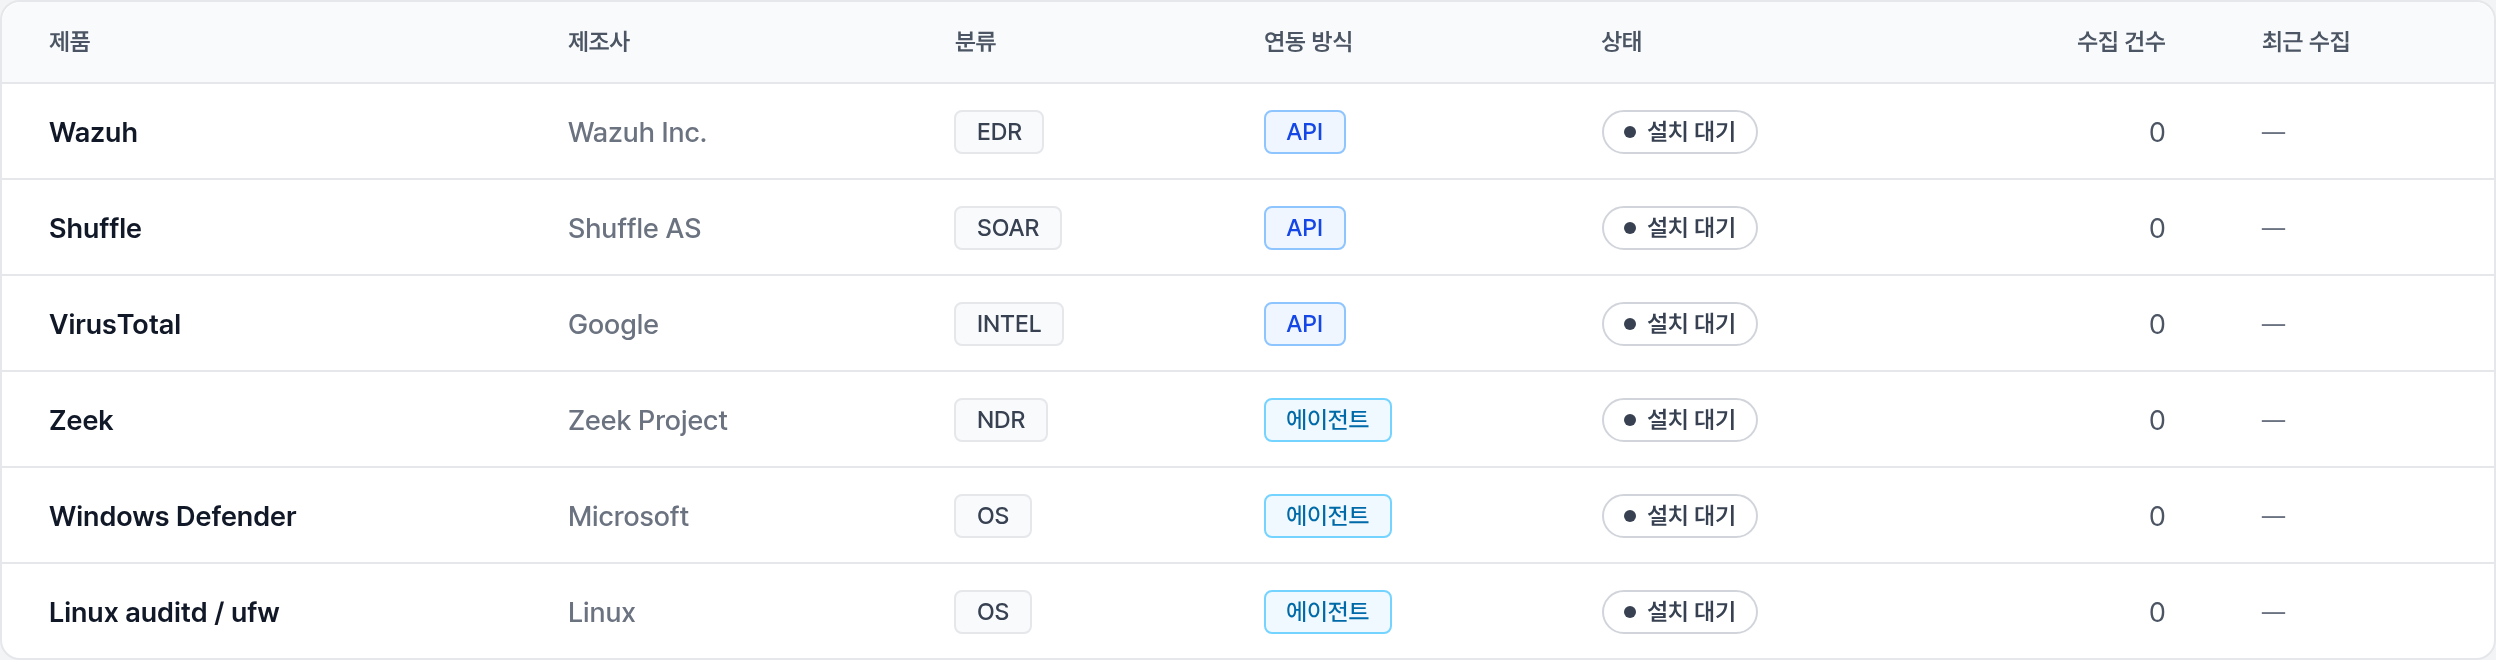
\includegraphics[width=0.9\textwidth]{screenshots-bas/integrations.png}
\caption{연동 목록(시험 환경에서는 아직 연결된 제품이 없음)}
\label{fig:integrations}
\end{figure}


\subsection{로그 정규화}\label{subsec:integ-normalize}

수집된 기록은 제품마다 형식이 다르므로 출처, 심각도, 요약 메시지 및 사건 발생 시각을 추출하여 공통 형식으로 변환하고, 원본 로그도 함께 저장한다.
사건 발생 시각과 플랫폼의 로그 수신 시각은 구분하여 저장한다.
수집기는 여러 건의 기록을 묶어서 전송하며, 이 과정에서 기록의 순서가 바뀌거나 전송이 수 초 지연될 수 있다. 따라서 이후 공격 실행 결과와 탐지 기록 간의 시간적 상관관계를 분석할 때에는 수신 시각이 아닌 실제 발생 시각을 사용해야 한다.
